\documentclass{standalone}
\usepackage{tikz}
\usetikzlibrary{patterns, positioning}
\usepackage[sfdefault]{ClearSans} %% option 'sfdefault' activates Clear Sans as the default text font
\usepackage[T1]{fontenc}

\begin{document}
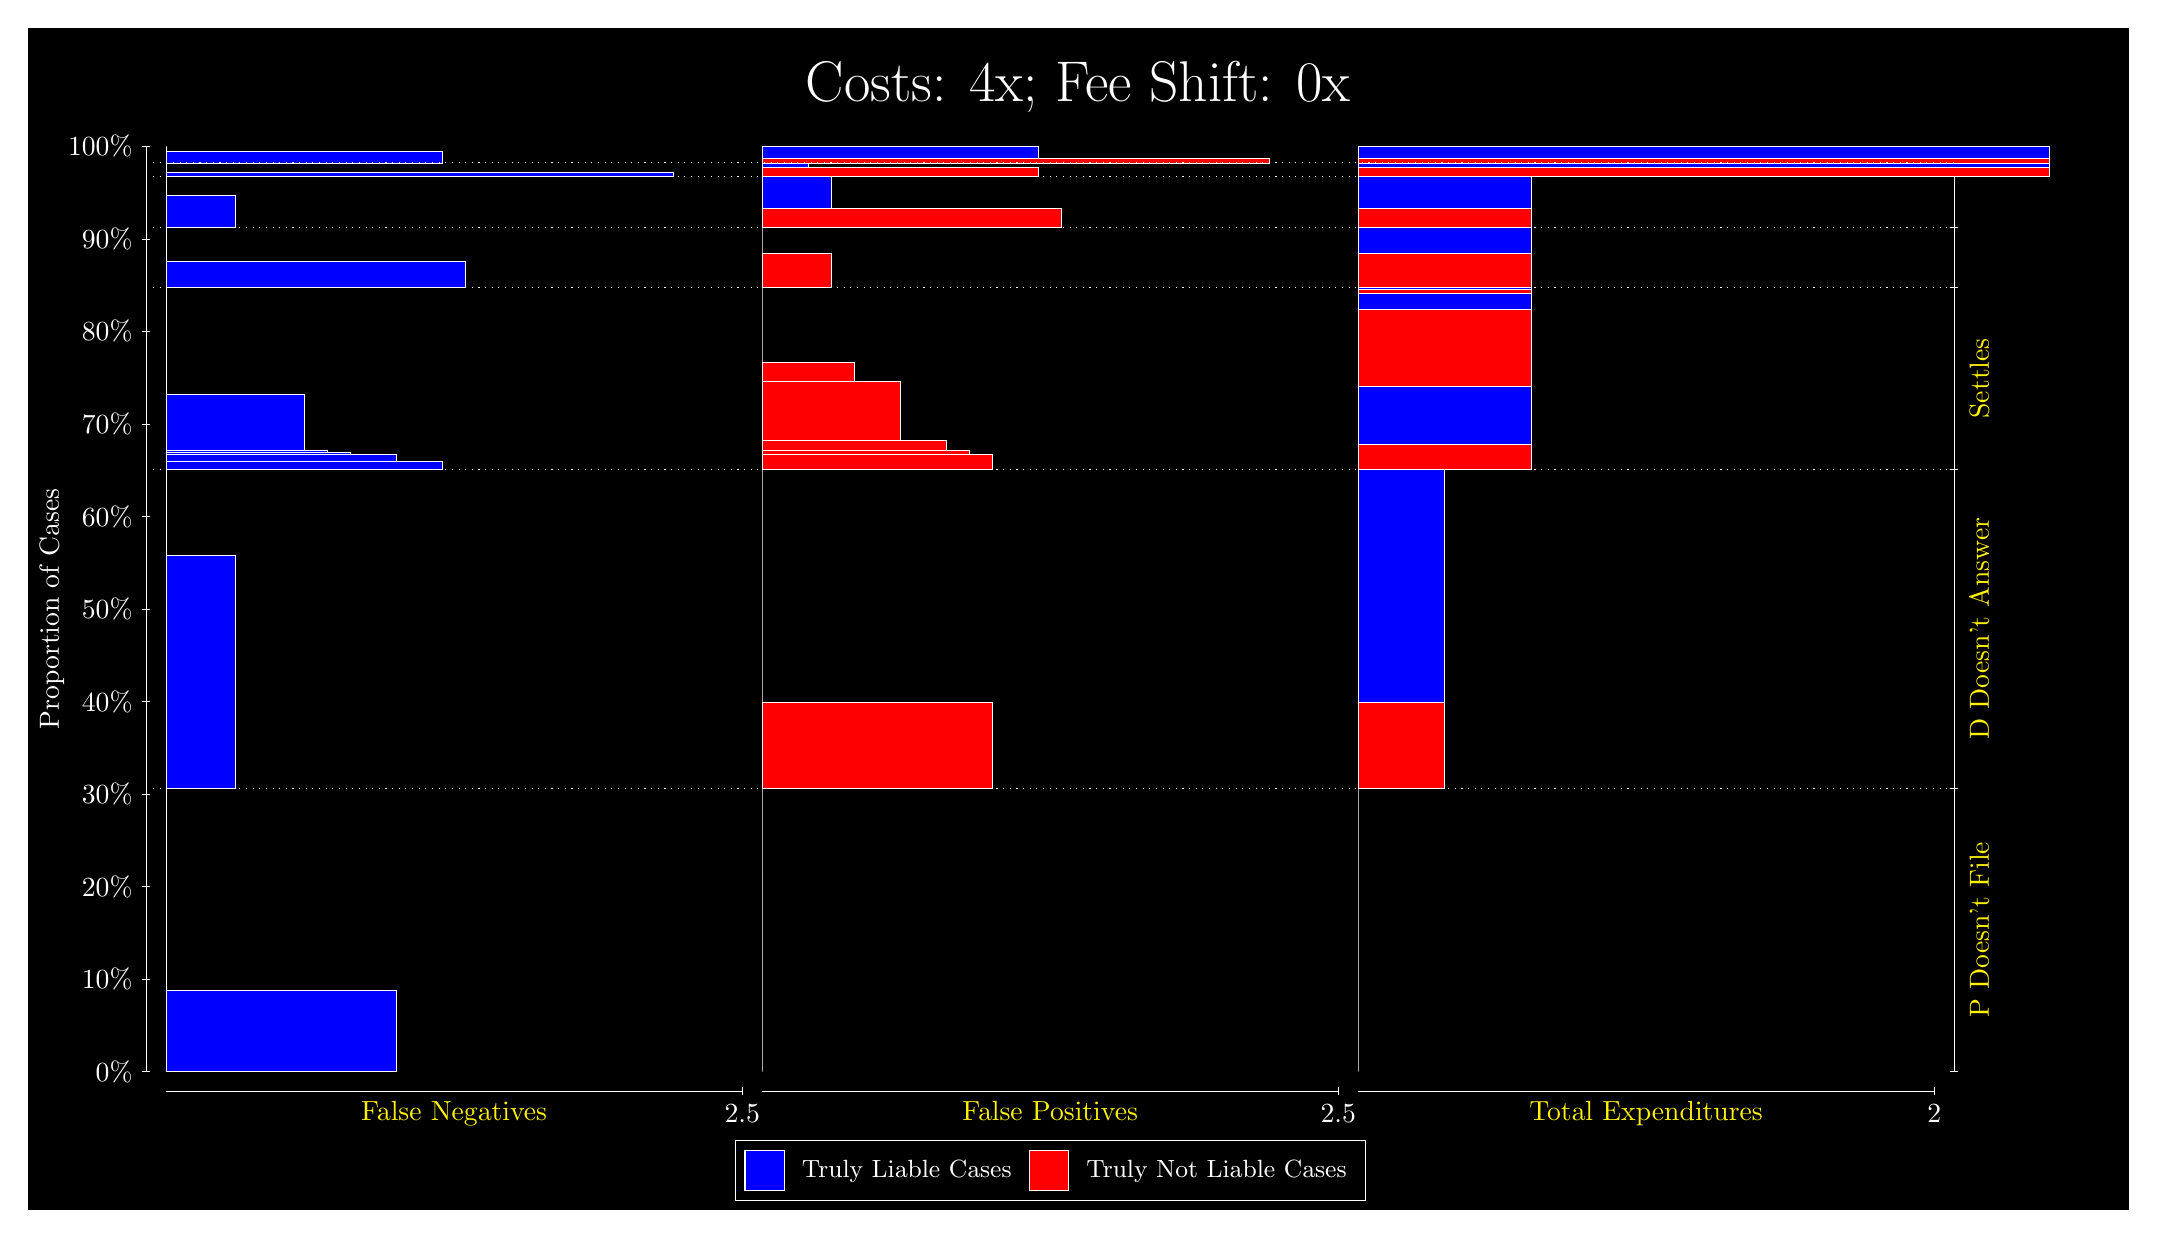
\begin{tikzpicture}
\draw[fill=black] (0,0) rectangle (26.667,15);
\draw[text=white] (0,13.5) rectangle (26.667,15) node[midway] {\huge Costs: 4x; Fee Shift: 0x};
\draw[white, very thin] (1.5,1.75) -- (1.5,13.5);
\node[rotate=90, text=white, anchor=center] at (0.3, 7.625) {Proportion of Cases};
\draw[white, very thin] (1.45,1.75) -- (1.55,1.75);
\node[text=white, anchor=east] at (1.45, 1.75) {0\%};
\draw[white, very thin] (1.45,2.925) -- (1.55,2.925);
\node[text=white, anchor=east] at (1.45, 2.925) {10\%};
\draw[white, very thin] (1.45,4.1) -- (1.55,4.1);
\node[text=white, anchor=east] at (1.45, 4.1) {20\%};
\draw[white, very thin] (1.45,5.275) -- (1.55,5.275);
\node[text=white, anchor=east] at (1.45, 5.275) {30\%};
\draw[white, very thin] (1.45,6.45) -- (1.55,6.45);
\node[text=white, anchor=east] at (1.45, 6.45) {40\%};
\draw[white, very thin] (1.45,7.625) -- (1.55,7.625);
\node[text=white, anchor=east] at (1.45, 7.625) {50\%};
\draw[white, very thin] (1.45,8.8) -- (1.55,8.8);
\node[text=white, anchor=east] at (1.45, 8.8) {60\%};
\draw[white, very thin] (1.45,9.975) -- (1.55,9.975);
\node[text=white, anchor=east] at (1.45, 9.975) {70\%};
\draw[white, very thin] (1.45,11.15) -- (1.55,11.15);
\node[text=white, anchor=east] at (1.45, 11.15) {80\%};
\draw[white, very thin] (1.45,12.325) -- (1.55,12.325);
\node[text=white, anchor=east] at (1.45, 12.325) {90\%};
\draw[white, very thin] (1.45,13.5) -- (1.55,13.5);
\node[text=white, anchor=east] at (1.45, 13.5) {100\%};

\draw[white, very thin] (24.457,1.75) -- (24.457,13.5);
\draw[white, very thin] (24.407,1.75) -- (24.507,1.75);
\node[anchor=west] at (24.407, 1.75) {};
\draw[white, very thin] (24.407,5.3487) -- (24.507,5.3487);
\node[anchor=west] at (24.407, 5.3487) {};
\draw[white, very thin] (24.407,9.3982) -- (24.507,9.3982);
\node[anchor=west] at (24.407, 9.3982) {};
\draw[white, very thin] (24.407,11.707) -- (24.507,11.707);
\node[anchor=west] at (24.407, 11.707) {};
\draw[white, very thin] (24.407,12.473) -- (24.507,12.473);
\node[anchor=west] at (24.407, 12.473) {};
\draw[white, very thin] (24.407,13.117) -- (24.507,13.117);
\node[anchor=west] at (24.407, 13.117) {};
\draw[white, very thin] (24.407,13.291) -- (24.507,13.291);
\node[anchor=west] at (24.407, 13.291) {};
\draw[white, very thin] (24.407,13.5) -- (24.507,13.5);
\node[anchor=west] at (24.407, 13.5) {};

\draw[white, very thin, fill=blue] (1.75,1.75) rectangle (4.6775,2.7757);
\draw[white, very thin, fill=red] (1.75,2.7757) rectangle (1.75,5.3487);
\draw[white, very thin, fill=blue] (1.75,5.3487) rectangle (2.6283,8.3042);
\draw[white, very thin, fill=red] (1.75,8.3042) rectangle (1.75,9.3982);
\draw[white, very thin, fill=blue] (1.75,9.3982) rectangle (5.2631,9.4991);
\draw[white, very thin, fill=blue] (1.75,9.4991) rectangle (4.6775,9.5925);
\draw[white, very thin, fill=blue] (1.75,9.5925) rectangle (4.092,9.6167);
\draw[white, very thin, fill=blue] (1.75,9.6167) rectangle (3.7993,9.6447);
\draw[white, very thin, fill=blue] (1.75,9.6447) rectangle (3.5065,10.348);
\draw[white, very thin, fill=red] (1.75,10.348) rectangle (1.75,11.707);
\draw[white, very thin, fill=blue] (1.75,11.707) rectangle (5.5558,12.042);
\draw[white, very thin, fill=red] (1.75,12.042) rectangle (1.75,12.473);
\draw[white, very thin, fill=blue] (1.75,12.473) rectangle (2.6283,12.872);
\draw[white, very thin, fill=red] (1.75,12.872) rectangle (1.75,13.117);
\draw[white, very thin, fill=blue] (1.75,13.117) rectangle (8.1906,13.173);
\draw[white, very thin, fill=red] (1.75,13.173) rectangle (1.75,13.291);
\draw[white, very thin, fill=blue] (1.75,13.291) rectangle (5.2631,13.443);
\draw[white, very thin, fill=red] (1.75,13.443) rectangle (1.75,13.5);
\draw[white, very thin, fill=red] (9.3189,1.75) rectangle (9.3189,4.3231);
\draw[white, very thin, fill=blue] (9.3189,4.3231) rectangle (9.3189,5.3487);
\draw[white, very thin, fill=red] (9.3189,5.3487) rectangle (12.246,6.4428);
\draw[white, very thin, fill=blue] (9.3189,6.4428) rectangle (9.3189,9.3982);
\draw[white, very thin, fill=red] (9.3189,9.3982) rectangle (12.246,9.5915);
\draw[white, very thin, fill=red] (9.3189,9.5915) rectangle (11.954,9.6418);
\draw[white, very thin, fill=red] (9.3189,9.6418) rectangle (11.661,9.7716);
\draw[white, very thin, fill=red] (9.3189,9.7716) rectangle (11.075,10.515);
\draw[white, very thin, fill=red] (9.3189,10.515) rectangle (10.49,10.757);
\draw[white, very thin, fill=blue] (9.3189,10.757) rectangle (9.3189,11.707);
\draw[white, very thin, fill=red] (9.3189,11.707) rectangle (10.197,12.137);
\draw[white, very thin, fill=blue] (9.3189,12.137) rectangle (9.3189,12.473);
\draw[white, very thin, fill=red] (9.3189,12.473) rectangle (13.125,12.717);
\draw[white, very thin, fill=blue] (9.3189,12.717) rectangle (10.197,13.117);
\draw[white, very thin, fill=red] (9.3189,13.117) rectangle (12.832,13.234);
\draw[white, very thin, fill=blue] (9.3189,13.234) rectangle (9.9044,13.291);
\draw[white, very thin, fill=red] (9.3189,13.291) rectangle (15.759,13.348);
\draw[white, very thin, fill=blue] (9.3189,13.348) rectangle (12.832,13.5);
\draw[white, very thin, fill=red] (16.888,1.75) rectangle (16.888,4.3231);
\draw[white, very thin, fill=blue] (16.888,4.3231) rectangle (16.888,5.3487);
\draw[white, very thin, fill=red] (16.888,5.3487) rectangle (17.986,6.4428);
\draw[white, very thin, fill=blue] (16.888,6.4428) rectangle (17.986,9.3982);
\draw[white, very thin, fill=red] (16.888,9.3982) rectangle (19.083,9.7212);
\draw[white, very thin, fill=blue] (16.888,9.7212) rectangle (19.083,10.449);
\draw[white, very thin, fill=red] (16.888,10.449) rectangle (19.083,11.435);
\draw[white, very thin, fill=blue] (16.888,11.435) rectangle (19.083,11.629);
\draw[white, very thin, fill=red] (16.888,11.629) rectangle (19.083,11.679);
\draw[white, very thin, fill=blue] (16.888,11.679) rectangle (19.083,11.707);
\draw[white, very thin, fill=red] (16.888,11.707) rectangle (19.083,12.137);
\draw[white, very thin, fill=blue] (16.888,12.137) rectangle (19.083,12.473);
\draw[white, very thin, fill=red] (16.888,12.473) rectangle (19.083,12.717);
\draw[white, very thin, fill=blue] (16.888,12.717) rectangle (19.083,13.117);
\draw[white, very thin, fill=red] (16.888,13.117) rectangle (25.67,13.234);
\draw[white, very thin, fill=blue] (16.888,13.234) rectangle (25.67,13.291);
\draw[white, very thin, fill=red] (16.888,13.291) rectangle (25.67,13.348);
\draw[white, very thin, fill=blue] (16.888,13.348) rectangle (25.67,13.5);
\draw[white, dotted] (1.5,5.3487) -- (24.457,5.3487);
\draw[white, dotted] (1.5,9.3982) -- (24.457,9.3982);
\draw[white, dotted] (1.5,11.707) -- (24.457,11.707);
\draw[white, dotted] (1.5,12.473) -- (24.457,12.473);
\draw[white, dotted] (1.5,13.117) -- (24.457,13.117);
\draw[white, dotted] (1.5,13.291) -- (24.457,13.291);
\draw[white, very thin] (1.75,1.5) -- (9.0689,1.5);
\node[text=yellow, anchor=north] at (5.4094, 1.5) {False Negatives};
\draw[white, very thin] (9.0689,1.45) -- (9.0689,1.55);
\node[text=white, anchor=north] at (9.0689, 1.45) {2.5};

\draw[white, very thin] (9.3189,1.5) -- (16.638,1.5);
\node[text=yellow, anchor=north] at (12.978, 1.5) {False Positives};
\draw[white, very thin] (16.638,1.45) -- (16.638,1.55);
\node[text=white, anchor=north] at (16.638, 1.45) {2.5};

\draw[white, very thin] (16.888,1.5) -- (24.207,1.5);
\node[text=yellow, anchor=north] at (20.547, 1.5) {Total Expenditures};
\draw[white, very thin] (24.207,1.45) -- (24.207,1.55);
\node[text=white, anchor=north] at (24.207, 1.45) {2};

\node[text=yellow, centered, rotate=90] at (24.777, 3.5494) {P Doesn't File};
\node[text=yellow, centered, rotate=90] at (24.777, 7.3735) {D Doesn't Answer};
\node[text=yellow, centered, rotate=90] at (24.777, 10.553) {Settles};





\draw (12.978300999999998,1.5) node[draw=none] (baseCoordinate) {};
\begin{scope}[align=center]
        \matrix[scale=0.5, draw=white, below=0.5cm of baseCoordinate, nodes={draw}, column sep=0.1cm]{
            \node[rectangle, draw, minimum width=0.5cm, minimum height=0.5cm, fill=blue] {}; &
            \node[draw=none, font=\small, text=white] (B) {Truly Liable Cases}; &
            \node[rectangle, draw, minimum width=0.5cm, minimum height=0.5cm, fill=red] {}; &
            \node[draw=none, font=\small, text=white] (B) {Truly Not Liable Cases}; \\
            };
\end{scope}

\end{tikzpicture}
\end{document}